% !TeX spellcheck = en_US
% This is LLNCS.DOC the documentation file of
% the LaTeX2e class from Springer-Verlag
% for Lecture Notes in Computer Science, version 2.4
\documentclass{llncs}
\usepackage{llncsdoc}
\usepackage{graphicx} 
\usepackage{booktabs}
\usepackage{amsmath}
\usepackage{amssymb}

\usepackage[linesnumbered,ruled]{algorithm2e}

\usepackage[noend]{algpseudocode}

\newcommand{\R}{\mathbb{R}}
%
\begin{document}
\thispagestyle{empty}
\rule{\textwidth}{1pt}
\vspace{2pt}
\begin{flushright}
\Huge
\begin{tabular}{@{}l}
Barriers to the\\
implementation of\\
k-anonymity and\\
related microdata\\
anonymization techniques\\
in a realworld application\\[6pt]

\end{tabular}
\end{flushright}
\rule{\textwidth}{1pt}
\vfill
\title{Barriers to the implementation of k-anonymity and related microdata anonymization techniques in a realworld application}
\author{Andreas Wiegnand, 1878334\\
	Ludwig Schallner, 1850413}
\institute{}
\maketitle
%
%\tableofcontents
\section*{Abstract}
ToDo: Abstract
\newpage
\setcounter{page}{1}

\section{Introduction}
%
Nowadays data is a key factor in nearly every domain. It is comparable to the gold rush of the \ensuremath{19^{th}.} century \cite{datarevo}. Furthermore, storage space and network ability increasingly become affordable \cite{sweeney2002k}. 
This is leading to the situation that the created and stored data is often not only useful to the original data holder, but to other researchers. Also, some data is only useful if its get shared with other data and get together analyzed. But those data may contain some personal or sensitive information. Such that the data should only get releases if the privacy is protected \cite{li2006achieving}.\\
\begin{table}[]
	\centering
	\caption{Basic example}
	\label{intro_example}
	\begin{tabular}{@{}llll@{}}
		\toprule
		SSN         & Age & Postcode & Problem         \\ \midrule
		680-90-2665 & 25  & 4568     & procrastination \\
		008-07-4179 & 34  & 4567     & stress          \\
		391-05-7998 & 48  & 4569     & stomach cancer  \\
		078-36-3853 & 39  & 4568     & obesity         \\
		411-71-9290 & 42  & 4561     & stomach ulcers  \\
		527-59-1948 & 27  & 4568     & stress          \\ \bottomrule
	\end{tabular}
\end{table}

Data like in table \ref{intro_example} have to get anonymized before it gets released. A very common
technique archive this goal is the so-called k-anonymity, which will prevent
the possibility that information about the individual gets leaked. This paper will
show the barriers to implementing k-anonymity. In Section
1 explains the mandatory basic to understand k-anonymity and its purpose.
Section 2 will discuss the underlying barriers of k-anonymity.
In Section 3 we will explain, possible attacks which also have to be considered as barriers for k-anonymity. Section 4 will show multiple algorithms to implement
k-anonymity. A summary of the whole paper will be in the last section
\newpage
\section{Basics}
In the following subsections basics will be explained. 
\subsubsection{Microdata:}
First of all, those data is containing records of information about individuals. The upside versus the more known summary or aggregate data is, that microdata is naturally flexible. Everyone who has this data can perform own statistics from that data \cite{microdataweb}.
\subsubsection{Identifier:}
They are attributes which can identify the record owner explicitly without any other attribute. For example the full name (first name and last name), telephone number, social security number, and more \cite{domingo2008critique}.
\subsubsection{Quasi-identifier:}
Even though explicit identifier got removed from published data (to anonymize the data). Attributes which non-explicitly identify the record owner are left. But if they get combined with other non-explicit attributes or other tables, they can reidentify the record owner. In such a case those combination of attributes are called quasi-identifier. For example Gender, Age, Postcode, weight and height \cite{dalenius1986finding}. Such process is shown in figure (the quasi-identifier would be the ZIP, birth date and sex) \ref{quasiidentifier}.
\begin{figure}[]
	\centering
	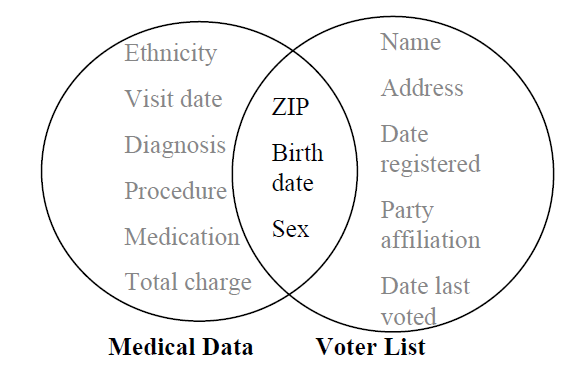
\includegraphics[width=0.6\textwidth]{linkingdata.png}
	\caption{Quasi-identifiers}%
	\label{quasiidentifier}
\end{figure}
\subsubsection{Sensitive data:}
Data which is useful for example researchers but are too private and should not be known publicly nor be accessible for outsiders. This is the data which the record owner do not want to get linked to.\cite{ldiversity}.

\subsubsection{Background-knowledge:}
Because its unknown what the attackers knows, we have to assume additionally to that he have access to table, the attackers knows that the table is generalized (to guarantee k-anonymity). Furthermore, the attacks is aware of the domain of the attributes.\\
\textbf{Instance-level background knowledge:}
The adversary knows about specific details about his target. For example Alice (the adversary) knows that Bob do not suffer from a disease, because he does not show the symptoms. In this case Alice may can conclude what Bob is really suffers from.\\
\textbf{Demographic background knowledge:}
The Adversary knows more general fact, for example P(t[condition] = cancer| t[Age] $\geq$ 40). With this information the attacker may use it to interference about records \cite{ldiversity}

\subsubsection{K-Anonymity:}
The goal of making a k-anonymized table, is to have at least (k-1) tuples of each identical tuple taking the corresponding quasi-identifiers into account \cite{sweeney2002k,li2006achieving}. For example the 2-anonyminized version of the table \ref{intro_example} in the introduction section would be the following table:
\begin{table}[]
	\centering
	\caption{Basic example 2-anonymized}
	\label{intro_example_sol}
	\begin{tabular}{@{}llll@{}}
		\toprule
		SSN         & Age & Postcode & Problem         \\ \midrule
		* & 2*  & 456*     & stress \\
		* & 3*  & 456*     & stress          \\
		* & 4*  & 456*     & stomach cancer  \\
		* & 3*  & 456*     & obesity         \\
		* & 4*  & 456*     & stomach ulcers  \\
		* & 2*  & 456*     & stress          \\ \bottomrule
	\end{tabular}
\end{table}\\
\textbf{Disclosure:} There are two kinds, \textbf{identity disclosure} if this is happening an individual gets linked to a particular record. Because of that \textbf{attribute disclosure} may happens, this is if new information about an individual gets reveled. For example, Bob gets linked to his record in \ref{intro_example_sol}, because of some attack (see Section 3.3). The adversary learns that he is suffering from stress \cite{sweeney2002k}.  
\subsubsection{Equivalence class:}
Is a set of all tuples with the identical quasi-identifiers of a table \cite{li2006achieving}.
\subsubsection{Global recoding/domain generalisation:}
This generalization technique is very common, if a attribute value get generalized then all occourences of that value gets replaced by the generalized one \cite{sweeney2002k,sweeney2002achieving,li2006achieving,incognito}. 
\subsubsection{Local recoding:}
This coding strategies works differently from the above described one. Local recording generalizes attribute values in cells. Because of that this strategies doesn't over generalize the table and the data distortion is significantly lower \cite{li2006achieving}. 

%\section{Theoretical and heuristically implantation of K-Anonymity}
%Another problem we will introduce is, that the producing of k-anonymity of a computational view is an NP-hard problem, like Meyersond and Williams shown.
 
\section{Underlying Barriers}

In the following section, we will show the basic and most challenging barriers to the implementation of k-Anonymity. First, we will show the barrier which appears if you k-anonymize the data, the so-called \textbf{distortion} of data, in some papers it also mentioned as data loss. 
%checked
\subsection{Distortion of data as Barrier} 
A basic underlying barrier of k-anonymity is, how to measure if a implementation has been successful or leads to a satisfying result. This can be measured by a simple calculation.
The \textbf{modification rate} is representing the fraction of cells which got modified within the attribute set of the quasi-identifier \cite{li2006achieving}.

	
\begin{table}[]
	\centering
	\caption{a: original table, b: example for local recording, c: example for domain generalization }
	\label{table_distortion}
	\begin{tabular}{@{}lllllllllll@{}}
		\multicolumn{3}{c}{\textbf{a}} &           & \multicolumn{3}{c}{\textbf{b}} &  & \multicolumn{3}{c}{\textbf{c}} \\ \midrule
		Gender  & Birthday   & Problem & \textbf{} & Gender  & Birthday   & Problem &  & Gender  & Birthday  & Problem  \\ \midrule
		male    & 13.08.1962 & stress  &           & male    & 13.08.1962 & stress  &  & *       & 196*      & stress   \\
		male    & 28.10.1967 & obesity &           & male    & 28.10.1967 & obesity &  & *       & 196*      & obesity  \\
		male    & 20.01.1977 & stress  &           & *       & 197*       & stress  &  & *       & 197*      & stress   \\
		female  & 15.09.1973 & obesity &           & *       & 197*       & obesity &  & *       & 197*      & obesity  \\
		female  & 15.03.1985 & stress  &           & female  & 15.03.1985 & stress  &  & *       & 198*      & stress   \\
		female  & 28.05.1986 & obesity &           & female  & 28.05.1986 & obesity &  & *       & 198*      & obesity  \\ \bottomrule
	\end{tabular}
\end{table}

\textbf{Example:} for table \ref{table_distortion}b, the modification rate is  33,$\overline{33}$\% (4 out of 12 quasi-identifier got changed) for table \ref{table_distortion}c: its is 100\% (12 out of 12 quasi-identifier got changed). Like this simple example shows the modification rate calculation is a unsatisfying procedure. Because of that the \textbf{weighted hierarchical distance} got introduced by Li, Wong, Fu and Pei. 
To calculate the \textbf{weighted hierarchical distance} of a cell, which got generalized from level p to level q, following formula is used \cite{li2006achieving}.\\
\scalebox{1.25}{$ WHD (p, q) = \frac{\sum_{j=q+1}^{p} \omega_{j,j-1}}{\sum_{j=2}^{h} \omega_{j,j-1}} $}\cite{li2006achieving}\\
Let the hierarchy of birth date be \{D/M/Y, M/Y, Y, 10Y, C/T/G/P, *\}. Where D/M/Y  would be day.month.year, 10Y a 10 years interval and C/T/G/R for Child/Teen/Grownup/Pensioner.\\

\textbf{Example with uniformed weight $w_{j,j-1} = 1$ where $2\leq j \leq h$} \cite{li2006achieving}: For the above example Birthday gets generalized from D/M/Y to 10Y, which corresponds into $WHD_{Birthday}(6,3) = \frac{3}{5} = 0,6$. For the Gender generalization it would be $WHD_{gender}(2,1) = \frac{1}{1} = 1$. Which means for generalize 5 cells of age from D/M/Y to 10Y one will have the same data distortion as if 3 cells of gender gets generalized from Male/Female to *. This calculation shows a much better way to address the distortion of data than the \textbf{modification rate} but it does not take how near a generalization is to the root (which would be *).\\

\textbf{Example with height weight: $w_{j,j-1} = 1 / (j-1)^{\beta}$ where 2 $\leq$ j $\leq$ h and $\beta = \R \geq$ 1} \cite{li2006achieving}:
$\beta$ would be chosen by the user. For example $\beta = 1$. For $WHD_{Birthday}(6,3) = \frac{0,\overline{33}+0,25+0,20}{1+0.5+0,\overline{33}+0,25+0,20} \sim 0,3431$. For $WHD_{gender}(2,1) = \frac{1}{1} = 1$. The distortion of nearly 3 changed cell of birthday from D/M/Y to  10Y have the same amount as if one cell of gender, from Female/Male to *, gets generalized. 

\subsubsection{Conclusion}

Because research need the information out of the tables, like of the examples. Its very important that as less as necessary information gets lost during the anonymization process. To show the importance  of this an additionally example, consider a table with surviver of a \textbf{idiom disaster beyond all expectations}. Researchers trying to find out the long-time effects of this disaster. Thats why the want to find out if victims get more likely to life a long and happy life if the live far away or close to the disasters location. If the data gets to much generalized by location its maybe useless for researchers to work with.

\subsection{Attacks as Barrier}

Furthermore, also attacks have to be considered as barriers to the implementation because if the implementation ignores the weaknesses which the attacks
use, k-anonymity will be useless. It is absolutely necessary that an attacker, under no circumstances, can learn about whatsoever target if he is studying the
published database. Not even if the attacker has background knowledge from
any other sources \cite{Dalenius1977}. Unfortunately like Dwork showed 2006 that such safety is impossible because of the impossibility to predict what the attacker may know. Therefore its important and necessary that the implementation takes possible attacks into account and implement countermeasures, but because attacks are not the main part of this paper it will be only a short introduction. 

\subsubsection{Homogeneity attack}

As an example, let Alice be the adversary and let be Bob her target. They are neighbors, someday Bob get transported with an ambulance to a hospital. Assume the hospital published the table \ref{homogenityattack}, where all current patients with them Nationality, Age, ZIP, and Problem are listed, but this table got 4-anonymized before release. Alice knows that Bob is a 31 old, American who lives in ZIP Code 02239. She can conclude that either he is entry 3, 5,6, or 11. Furthermore, all of these entry have the same Problem, Cancer. Alice can conclude Bob is suffering from Cancer even if the table the table got 4-anonymized \cite{sweeney2002k,ldiversity}. To counter such attacker \textbf{diversity} is needed \cite{ldiversity}. Such method is the so-called l-diversity which will not discuss further in this paper.  

% Please add the following required packages to your document preamble:
% \usepackage{booktabs}
\begin{table}[]
	\centering
	\caption{Homogeneity attack}
	\label{homogenityattack}
	\begin{tabular}{@{}llllllllll@{}}
		\cmidrule(lr){2-5} \cmidrule(l){7-10}
		& Nationality     & Age & ZIP   & Problem         &  & Nationality & Age      & ZIP   & Problem         \\ \cmidrule(lr){2-5} \cmidrule(l){7-10} 
		1  & American        & 42  & 02135 & Viral Infect    &  & *           & $\geq$40 & 021** & Viral Infect    \\
		2  & Japanese        & 41  & 02133 & Hearth disease  &  & *           & $\geq$40 & 021** & Hearth disease  \\
		3  & Germany         & 38  & 02238 & Hearth disease  &  & *           & 3*       & 0223* & Cancer          \\
		4  & Japanese        & 29  & 02139 & Fever           &  & *           & $\leq$30 & 021** & Fever           \\
		5  & Indina          & 37  & 02232 & Viral Infection &  & *           & 3*       & 0223* & Cancer          \\
		6  & Native-american & 34  & 02236 & Cancer          &  & *           & 3*       & 0223* & Cancer          \\
		7  & Russia          & 53  & 02138 & Viral Infection &  & *           & $\geq$40 & 021** & Viral Infection \\
		8  & China           & 23  & 02139 & Cancer          &  & *           & $\leq$30 & 021** & Cancer          \\
		9  & American        & 23  & 02141 & Short of breath &  & *           & $\leq$30 & 021** & Short of breath \\
		10 & Indian          & 46  & 02139 & Viral Infection &  & *           & $\geq$40 & 021** & Viral Infection \\
		11 & American        & 31  & 02239 & Vomiting        &  & *           & 3*       & 0223* & Cancer          \\
		12 & American        & 28  & 02130 & Viral Infection &  & *           & $\leq$30 & 021** & Viral Infection \\ \cmidrule(lr){2-5} \cmidrule(l){7-10} 
	\end{tabular}
\end{table}

\subsubsection{Background knowledge attack}
This attack uses the demographic background knowledge, which got explained in the basics, of an adversary. Assume Alice have a college, which gets also to the same hospital. This college is 32 years old, Japanese and has the ZIP 93607. Everyone with the same quasi-identifiers (Age = 3* and ZIP = 936**) have cancer or a heart disease. Because she knows that Japanese have a very low risk of a heart disease she concludes her college has cancer \cite{ldiversity}.
\begin{table}[]
	\centering
	\caption{Background Knowledge Attack}
	\label{tablebackground}
	\begin{tabular}{@{}llllllll@{}}
		\cmidrule(r){1-4} \cmidrule(l){6-8}
		& ZIP Code & Age & Disease        &  & ZIP Code & Age      & Disease        \\ \cmidrule(r){1-4} \cmidrule(l){6-8} 
		1 & 93677    & 29  & Liver Disease   &  & 936**    & $\leq$30 & Liver Disease   \\
		2 & 93602    & 22  & Liver Disease   &  & 936**    & $\leq$30 & Liver Disease   \\
		3 & 93909    & 52  & Cancer         &  & 9390*    & $\geq$40 & Cancer         \\
		4 & 93906    & 47  & Flu            &  & 9390*    & $\geq$40 & Flu            \\
		5 & 93673    & 36  & Heart Disease &  & 936**    & 3*       & Heart Disease \\
		6 & 93607    & 32  & Cancer         &  & 936**    & 3*       & Cancer         \\ \cmidrule(r){1-4} \cmidrule(l){6-8} 
	\end{tabular}
\end{table}

\subsubsection{Unsorted matching attack against k-anonymity}
This attack is based on the very common strategy to release two tables separately. For example, assume a two column weight table (a). This table gets separated into two tables (b, c). Table b will contain Age completely generalized but ZIP ungeneralized, table c will have Age ungeneralized but Zip Generalized. The adversary just will merge both tables and will get the table (a), and get access to sensitive information. This weakness can be fixed via random sorting. \cite{sweeney2002k}.

\begin{table}[]
	\centering
	\caption{My caption}
	\label{my-label}
	\begin{tabular}{@{}cccccccc@{}}
		\multicolumn{2}{c}{\textbf{a}} & \multicolumn{1}{l}{} & \multicolumn{2}{c}{\textbf{b}} & \multicolumn{1}{l}{} & \multicolumn{2}{c}{\textbf{c}} \\ \cline{1-2} \cline{4-5} \cline{7-8} 
		Age           & ZIP            &                      & Age           & ZIP            &                      & Age           & ZIP            \\ \cline{1-2} \cline{4-5} \cline{7-8} 
		42            & 91058          &                      & *             & 91058          &                      & 42            & 91050          \\
		44            & 91058          &                      & *             & 91058          &                      & 44            & 91050          \\
		50            & 27785          &                      & *             & 27785          &                      & 50            & 27780          \\
		52            & 27785          &                      & *             & 27785          &                      & 52            & 27780          \\
		20            & 32105          &                      & *             & 32105          &                      & 20            & 32100          \\
		21            & 32105          &                      & *             & 32105          &                      & 21            & 32100          \\
		31            & 67676          &                      & *             & 67676          &                      & 31            & 67670          \\
		32            & 67676          &                      & *             & 67676          &                      & 32            & 67670          \\ \cline{1-2} \cline{4-5} \cline{7-8} 
	\end{tabular}
\end{table}

\subsubsection{Conclusion}
After showing possible attacks on k-anonymity it should be clear that before implementation an application with k-anonymity, these attacks should be tested and the application should be secure against any possible attack. 

\subsection{NP Hard}
Todo: why non polynomial problem?
\section{Algorithm}
This section will show some algorithms which goals is to archive k-anonymity through generalization. 

\subsection{The KACA Algorithm}
This algorithm idea is to archive k-anonymity by clustering attribute hierarchical structures. The algorithm choose a random equivalent class, which is smaller than k. The next step is to form a lager equivalent class by merging the chosen  one with the closest equivalent class. Which is resulting in a larger combined equivalent class. Through repeating this process the final result is that each equivalent class consists of at least k tuples  \cite{li2006achieving}.\\
\begin{algorithm}[H]
	\caption{K-Anonymization by Clustering in Attribute hierarchies (KACA) \cite{li2006achieving}}
	form equivalence classes from the data set\\
	\While{there exists an equivalence class of size $<$ k}{
	randomly choose an equivalence class $C$ of size $k$ k\\
	evaluate the pairwise distance of $C$ and all other equivalence classes\\
	find the equivalence class $C'$ with the smallest distance to $C$\\
	generalise the equivalence classes $C$ and $C'$
	}	
\end{algorithm}
This algorithm has a runtime of $O(nlogn + |E|^{2})$. Li, Wong, Fu, and Pei have shown that their KACA-Algorithm is resulting in a 5.57 times smaller amount of distortion as the well known Incognito algorithm. The reason is lying in the technique which Incognito is using. Its a global recoding algorithm, which is resulting in a over-generalized table \cite{li2006achieving}.
\subsection{The OlA Algorithm }
The OLA Algorithm works in 3 Steps that will now be explained.
\begin{enumerate}
	\item For every generalization, strategy builds a binary search to find all k-anonymous nodes in the different strategies.
	\item For every generalization strategy that includes k-anonymous nodes save the one with the least Information loss in the hole generalization strategy, this is referred to a local option k-anonymous solution.
	\item Now compare the local optimum solutions to respect of the information loss. The one with the lowest Information loss of all local optimum solutions is the global optimum solution.
\end{enumerate}
The most time-consuming operation is finding the all the K-anonymous notes with and compares them to each other with respect to their information loss.  To get a better performance at the Programm step 1) the OLA algorithm works with Predictive Tagging that boost the process.  This Tagging take advantage of 2 Theorems of the generalization Lattice. That every k-anonymous note in the same generalization lattice on hight n. All notes above n and in the same generalization strategy are also k-anonymous. So the algorithm only has to find the first k-anonymous note in the strategy and tag all above as k-anonymous.   

\subsection{Cloaking Algorithm}
Moving object data poses new challenges to a traditional database, data mining, and privacy-preserving technologies due to its unique characteristics: it is time-dependent, location-dependent, and is generated in large volumes of high-dimensional stream data. The following algorithm shows an example of privacy production.The Cloaking Algorithm tries to produce Anonymity on location-based data for users of Location Bases Services(LBS). The Cloaking Algorithm is installed on a location protection broker on a trusted server and anonymize messages which will afterward send the LBS. K-anonymity prevents such a privacy breach by ensuring that each individual record can only be released if there are at least k − 1 other (distinct) individuals whose associated records are indistinguishable from the former in terms of their quasi-identifier values. there a two possible attacks to get the identity of a sender of a message. At the  Restricted Space Identification, the attacker A observes that message M is sent from location L afterward he gets the background knowledge that L belongs to someone specific. For example, if Mr. Bob the owner of a flat sends a message and the attacker observes this message. He can re-link the identity of Bob. Another Attack is  Observation Identification. If A has observed the current location L of subject S and finds a message M from L then A learns that S has sent M.  To prevent this leaking of information the cloaking algorithm works with Spatial Cloaking and Temporal Cloaking. Spatial Cloakings goal is to increase the location of m in such a way that there are more messages in it. So that there is not only one message at a time in an area. Temporal Cloaking extends the sending time until more messages are in one area. 


%\section{Releated techniques}
\section{Summary}
Like we saw in section OLA algorithm there are possibilities of choosing between different information loss metrics which all compute different values to the same k-anonymous node. So the implementer has to choose which one fits the most in his data. Different Metrics have pros and cons and have to be compared. Another problem with Information loss is that you can measure the information loss on your dataset but what would be more is interesting the information loss compared to upcoming data mining tool or machine learning application. The information loss metrics can´t know which information is important for the upcoming data mining step.suppression can also harm the quality of the data and should be chosen wisely.The production of k-anonymity is NP-Hard which results in a difficult implementation in real-time applications like the Cloaking - Algorithm had shown. This Complexity can result in problems of finding an optimal solution in real-world data sets and can make a practical implementation difficult. High Dimensional Data like transaction data with more than thousand of attributes are in practice not capable to produce k-anonymity for all attributes. The reason for that is the so-called Curse of High Dimensionality which produces a metric space which is too large to produce k-anonymity solutions for all attributes. A  Possibility is so called, bounded background knowledge that some attributes can´t be used as a quasi-identifier because the effort of getting background knowledge which can be linked to the attributes is estimated too high. Like shown i chapter {Attacks as Barrier} attacks against k-anonymity are a threat for the anonymity of the user and can result in identity disclosure.There solutions regarding these kinds of attacks we proposed in this paper. L-Diversity and T-Closeness will help them. The cloaking algorithm shoves a good example of the connection between anonymity and usability. The anonymization of the data reduces the usability of location-based services. Which comes from the construction of the Spatial cloaking and Temporal cloaking boxes to have enough messages to constrain them and let the be k-anonymous. The Software gives the option that a user of the client can decide how much usability he wants to sacrifice to get anonymity. So the user is at least under the control of how much utility he wants to give up. 
\newpage
\bibliography{literature}
\bibliographystyle{splncs03}

\end{document}


